
\subsection{{Description}}

	{The 8-bit Arithmetic Logic Unit (ALU) is a crucial digital computing component, performing arithmetic and logic operations on 8-bit binary data.}
	
	{Its operations, including addition, subtraction, AND, OR, XOR, and bitwise shifts, depend on the specific problem set, as the microcode input-feedback mechanism can change, altering the order of operations to suit the problem at hand.}
	
	{Controlled by signals from the processor's control unit, the ALU's outputs serve as inputs to the seven-segment display unit, influencing subsequent stages in digital systems.}

\subsection{{Truth Table}}

	{The truth table for the ALU is dependent upon the specific problem set under consideration, as it reflects the varied input combinations and corresponding outputs dictated by the problem's computational requirements.}

\subsection{{Block Diagram}}

	\begin{figure}[H]
		\centering
		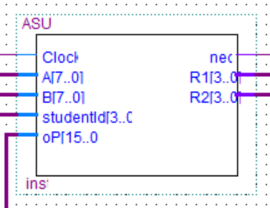
\includegraphics[width=10cm]{Pictures/ALU.png}
		\caption{{Block Diagram for Arithmetic Logic Unit}}
		\label{}
	\end{figure}


\subsection{{Timing Diagram}}

	{The timing diagram for the ALU is influenced by the problem set under consideration, as it adapts to the unique sequence and duration of operations required by the computational demands of the specific problem.}
